\documentclass{article}
\usepackage[german]{babel}
\usepackage{float}
\usepackage{fourier}
\usepackage[utf8]{inputenc}
\usepackage[T1]{fontenc}
\usepackage{amsfonts,amsthm, amsmath}
\usepackage{listings}
% The following is needed in order to make the code compatible
% with both latex/dvips and pdflatex.
\ifx\pdftexversion\undefined
\usepackage[dvips]{graphicx}
\else
\usepackage[pdftex]{graphicx}
\DeclareGraphicsRule{*}{mps}{*}{}
\fi

\setlength\parindent{0pt}
\lstset{language=Java}

\begin{document}

\textbf{Team:} TEAM 01, Falco Winkler (FW), Daniel Schruhl (DS)\\
\\
\textbf{Aufgabenteilung:}
\begin{itemize}
    \item IDL Compiler
    \item Namensdienst
    \item mware\_lib Library
\end{itemize}

\textbf{Quellenangaben:}
\begin{itemize}
    \item Aufgabe 4, 11.06.2017, C. Klauck \& H. Schulz: \newline
    http://users.informatik.haw-hamburg.de/~schulz/pub/Verteilte-Systeme/AI5-VSP/Aufgabe4/
\end{itemize}

\textbf{Bearbeitungszeitraum:}
\begin{itemize}
	\item 11.06.2017 4 Stunden (DS)
\end{itemize}

\textbf{Aktueller Stand:}
\begin{itemize}
	\item IDL Compiler begonnen
    \item Namensdienst
    \item mware\_lib Library
\end{itemize}

\textbf{Änderung des Entwurfs:}
\begin{itemize}
    \item Keine Änderungen
\end{itemize}

\newpage

\section{Einführung und Ziele}
Es soll eine einfache objektorientierte Middleware entworfen werden, die Methodenaufrufe
eines entfernten Objektes ermöglicht.

Zur Orientierung gilt hierbei die CORBA Architektur. Genauer soll hier ein ORB zur
Verfügung gestellt werden, der es ermöglicht Methoden von entfernten Objekten aufzurufen.

Zur Abstraktion und Beschreibung der Schnittstellen der Objekte soll eine IDL verwendet werden.
Diese IDL wird dann zur Erzeugung von Klassen- und Methodenrümpfen verwendet.

Außerdem beinhaltet der ORB einen Namensdienst, der Objektreferenzen in einem Netz mit Namen finden
kann.

Die Middleware an sich soll durch eine Library abstrahiert und verwendbar sein.

\subsection{Randbedingungen}
Der Namensdienst soll auf einem entfernten Rechner unabhängig von der Middleware Library
lauffähig sein. Der Port muss zur Laufzeit einstellbar sein.

Der IDL-Compiler soll in einem Package oder einer \texttt{.jar} Datei zur Verfügung gestellt
werden. Der Compiler soll folgende IDL Typen unterstützen:

\begin{itemize}
    \item module (keine Schachtelung, 1 Modul pro Datei)
    \item class (nicht als Parameter oder Returnwert, keine Schachtelung)
    \item int
    \item double
    \item string
\end{itemize}

Ein Beispiel:
\begin{lstlisting}
module math_ops {
  class Calculator {
   double add(double a, double b);
   string getStr(double a);
 };
};
\end{lstlisting}

Die Middleware Library soll in einem Package \texttt{mware\_lib} zusammengefasst werden.

Wenn eine Serverapplikation während eines entfernten Methodenaufrufes eine RuntimeException
wirft, soll diese an den Aufrufer weitergeleitet werden.

Es soll möglich sein, dass zwei oder mehrere Klienten die selbe Objektreferenz zeitgleich
nutzen wollen. Das soll innerhalb der Middleware nicht zu Deadlocks führen.

\subsection{Kontextbegrenzung}
Die Implementierung soll in Java vorliegen.

Die Behebung von Deadlocks in den Anwendungen ist nicht Aufgabe der Middleware.

\newpage

\section{Gesamtsystem}

\subsection{Bausteinsicht}
%\begin{figure}[H]
%    \centering
%    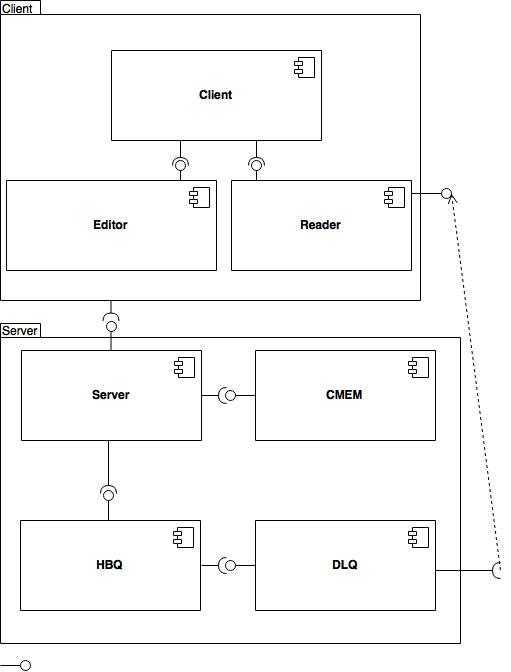
\includegraphics[width=0.5\textwidth]{component-diagram.png}
%    \caption[seq-dia]{Komponentendiagramm der ggT-App}
%    \label{fig:component-diagram}
%\end{figure}

\subsection{Laufzeitsicht}
%\begin{figure}[H]
%    \centering
%    \includegraphics[width=1.0\textwidth]{sequence-diagram.png}
%    \caption[seq-dia]{Eine ggT Berechnung mit Abbruch per Voting}
%    \label{fig:seq-diagram}
%\end{figure}

\newpage

\section{Subsysteme und Komponenten}

\end{document}